\documentclass[]{article}
\usepackage{lmodern}
\usepackage{amssymb,amsmath}
\usepackage{ifxetex,ifluatex}
\usepackage{fixltx2e} % provides \textsubscript
\ifnum 0\ifxetex 1\fi\ifluatex 1\fi=0 % if pdftex
  \usepackage[T1]{fontenc}
  \usepackage[utf8]{inputenc}
\else % if luatex or xelatex
  \ifxetex
    \usepackage{mathspec}
  \else
    \usepackage{fontspec}
  \fi
  \defaultfontfeatures{Ligatures=TeX,Scale=MatchLowercase}
\fi
% use upquote if available, for straight quotes in verbatim environments
\IfFileExists{upquote.sty}{\usepackage{upquote}}{}
% use microtype if available
\IfFileExists{microtype.sty}{%
\usepackage{microtype}
\UseMicrotypeSet[protrusion]{basicmath} % disable protrusion for tt fonts
}{}
\usepackage[margin=1in]{geometry}
\usepackage{hyperref}
\hypersetup{unicode=true,
            pdftitle={Conos SCTransformed sample 7},
            pdfauthor={Evelin Aasna},
            pdfborder={0 0 0},
            breaklinks=true}
\urlstyle{same}  % don't use monospace font for urls
\usepackage{color}
\usepackage{fancyvrb}
\newcommand{\VerbBar}{|}
\newcommand{\VERB}{\Verb[commandchars=\\\{\}]}
\DefineVerbatimEnvironment{Highlighting}{Verbatim}{commandchars=\\\{\}}
% Add ',fontsize=\small' for more characters per line
\usepackage{framed}
\definecolor{shadecolor}{RGB}{248,248,248}
\newenvironment{Shaded}{\begin{snugshade}}{\end{snugshade}}
\newcommand{\AlertTok}[1]{\textcolor[rgb]{0.94,0.16,0.16}{#1}}
\newcommand{\AnnotationTok}[1]{\textcolor[rgb]{0.56,0.35,0.01}{\textbf{\textit{#1}}}}
\newcommand{\AttributeTok}[1]{\textcolor[rgb]{0.77,0.63,0.00}{#1}}
\newcommand{\BaseNTok}[1]{\textcolor[rgb]{0.00,0.00,0.81}{#1}}
\newcommand{\BuiltInTok}[1]{#1}
\newcommand{\CharTok}[1]{\textcolor[rgb]{0.31,0.60,0.02}{#1}}
\newcommand{\CommentTok}[1]{\textcolor[rgb]{0.56,0.35,0.01}{\textit{#1}}}
\newcommand{\CommentVarTok}[1]{\textcolor[rgb]{0.56,0.35,0.01}{\textbf{\textit{#1}}}}
\newcommand{\ConstantTok}[1]{\textcolor[rgb]{0.00,0.00,0.00}{#1}}
\newcommand{\ControlFlowTok}[1]{\textcolor[rgb]{0.13,0.29,0.53}{\textbf{#1}}}
\newcommand{\DataTypeTok}[1]{\textcolor[rgb]{0.13,0.29,0.53}{#1}}
\newcommand{\DecValTok}[1]{\textcolor[rgb]{0.00,0.00,0.81}{#1}}
\newcommand{\DocumentationTok}[1]{\textcolor[rgb]{0.56,0.35,0.01}{\textbf{\textit{#1}}}}
\newcommand{\ErrorTok}[1]{\textcolor[rgb]{0.64,0.00,0.00}{\textbf{#1}}}
\newcommand{\ExtensionTok}[1]{#1}
\newcommand{\FloatTok}[1]{\textcolor[rgb]{0.00,0.00,0.81}{#1}}
\newcommand{\FunctionTok}[1]{\textcolor[rgb]{0.00,0.00,0.00}{#1}}
\newcommand{\ImportTok}[1]{#1}
\newcommand{\InformationTok}[1]{\textcolor[rgb]{0.56,0.35,0.01}{\textbf{\textit{#1}}}}
\newcommand{\KeywordTok}[1]{\textcolor[rgb]{0.13,0.29,0.53}{\textbf{#1}}}
\newcommand{\NormalTok}[1]{#1}
\newcommand{\OperatorTok}[1]{\textcolor[rgb]{0.81,0.36,0.00}{\textbf{#1}}}
\newcommand{\OtherTok}[1]{\textcolor[rgb]{0.56,0.35,0.01}{#1}}
\newcommand{\PreprocessorTok}[1]{\textcolor[rgb]{0.56,0.35,0.01}{\textit{#1}}}
\newcommand{\RegionMarkerTok}[1]{#1}
\newcommand{\SpecialCharTok}[1]{\textcolor[rgb]{0.00,0.00,0.00}{#1}}
\newcommand{\SpecialStringTok}[1]{\textcolor[rgb]{0.31,0.60,0.02}{#1}}
\newcommand{\StringTok}[1]{\textcolor[rgb]{0.31,0.60,0.02}{#1}}
\newcommand{\VariableTok}[1]{\textcolor[rgb]{0.00,0.00,0.00}{#1}}
\newcommand{\VerbatimStringTok}[1]{\textcolor[rgb]{0.31,0.60,0.02}{#1}}
\newcommand{\WarningTok}[1]{\textcolor[rgb]{0.56,0.35,0.01}{\textbf{\textit{#1}}}}
\usepackage{graphicx,grffile}
\makeatletter
\def\maxwidth{\ifdim\Gin@nat@width>\linewidth\linewidth\else\Gin@nat@width\fi}
\def\maxheight{\ifdim\Gin@nat@height>\textheight\textheight\else\Gin@nat@height\fi}
\makeatother
% Scale images if necessary, so that they will not overflow the page
% margins by default, and it is still possible to overwrite the defaults
% using explicit options in \includegraphics[width, height, ...]{}
\setkeys{Gin}{width=\maxwidth,height=\maxheight,keepaspectratio}
\IfFileExists{parskip.sty}{%
\usepackage{parskip}
}{% else
\setlength{\parindent}{0pt}
\setlength{\parskip}{6pt plus 2pt minus 1pt}
}
\setlength{\emergencystretch}{3em}  % prevent overfull lines
\providecommand{\tightlist}{%
  \setlength{\itemsep}{0pt}\setlength{\parskip}{0pt}}
\setcounter{secnumdepth}{0}
% Redefines (sub)paragraphs to behave more like sections
\ifx\paragraph\undefined\else
\let\oldparagraph\paragraph
\renewcommand{\paragraph}[1]{\oldparagraph{#1}\mbox{}}
\fi
\ifx\subparagraph\undefined\else
\let\oldsubparagraph\subparagraph
\renewcommand{\subparagraph}[1]{\oldsubparagraph{#1}\mbox{}}
\fi

%%% Use protect on footnotes to avoid problems with footnotes in titles
\let\rmarkdownfootnote\footnote%
\def\footnote{\protect\rmarkdownfootnote}

%%% Change title format to be more compact
\usepackage{titling}

% Create subtitle command for use in maketitle
\providecommand{\subtitle}[1]{
  \posttitle{
    \begin{center}\large#1\end{center}
    }
}

\setlength{\droptitle}{-2em}

  \title{Conos SCTransformed sample 7}
    \pretitle{\vspace{\droptitle}\centering\huge}
  \posttitle{\par}
    \author{Evelin Aasna}
    \preauthor{\centering\large\emph}
  \postauthor{\par}
      \predate{\centering\large\emph}
  \postdate{\par}
    \date{8/16/2019}


\begin{document}
\maketitle

\begin{Shaded}
\begin{Highlighting}[]
\NormalTok{norm =}\StringTok{ "SCT"}
\ControlFlowTok{if}\NormalTok{ (norm }\OperatorTok{==}\StringTok{ "log"}\NormalTok{)\{assay =}\StringTok{ "RNA"}\NormalTok{\}}
\ControlFlowTok{if}\NormalTok{ (norm }\OperatorTok{==}\StringTok{ "SCT"}\NormalTok{)\{assay =}\StringTok{ "SCT"}\NormalTok{\}}
\end{Highlighting}
\end{Shaded}

Created an integrated seurat object with 4 assays. Using subset of cells
from sample 07

\begin{Shaded}
\begin{Highlighting}[]
\KeywordTok{DefaultAssay}\NormalTok{(seu) <-}\StringTok{ }\NormalTok{assay}

\ControlFlowTok{if}\NormalTok{ (norm }\OperatorTok{==}\StringTok{ "log"}\NormalTok{)\{nPCA =}\StringTok{ }\DecValTok{20}\NormalTok{\}}
\ControlFlowTok{if}\NormalTok{ (norm }\OperatorTok{==}\StringTok{ "SCT"}\NormalTok{)\{nPCA =}\StringTok{ }\DecValTok{30}\NormalTok{\}}
\NormalTok{seu <-}\StringTok{ }\KeywordTok{RunPCA}\NormalTok{(seu, }\DataTypeTok{features =} \KeywordTok{VariableFeatures}\NormalTok{(seu) )}
\end{Highlighting}
\end{Shaded}

\begin{verbatim}
## Warning: Cannot add objects with duplicate keys (offending key: PC_),
## setting key to 'pca_'
\end{verbatim}

\begin{Shaded}
\begin{Highlighting}[]
\NormalTok{seu <-}\StringTok{ }\KeywordTok{RunTSNE}\NormalTok{(seu, }\DataTypeTok{dims =} \DecValTok{1}\OperatorTok{:}\NormalTok{nPCA )}
\NormalTok{seu <-}\StringTok{ }\KeywordTok{FindNeighbors}\NormalTok{(seu, }\DataTypeTok{dims =} \DecValTok{1}\OperatorTok{:}\NormalTok{nPCA)}
\end{Highlighting}
\end{Shaded}

\begin{verbatim}
## Computing nearest neighbor graph
\end{verbatim}

\begin{verbatim}
## Computing SNN
\end{verbatim}

\begin{Shaded}
\begin{Highlighting}[]
\NormalTok{seu <-}\StringTok{ }\KeywordTok{FindClusters}\NormalTok{(seu, }\DataTypeTok{verbose =} \OtherTok{FALSE}\NormalTok{)}
\end{Highlighting}
\end{Shaded}

Using 5000 most variably expressed decidua genes as reference.

Each dataset is clustered separately

\begin{Shaded}
\begin{Highlighting}[]
\CommentTok{# how many cores on HPC?}
\NormalTok{con <-}\StringTok{ }\NormalTok{Conos}\OperatorTok{$}\KeywordTok{new}\NormalTok{(seu_list, }\DataTypeTok{n.cores=}\DecValTok{4}\NormalTok{)}

\NormalTok{con}\OperatorTok{$}\KeywordTok{plotPanel}\NormalTok{(}\DataTypeTok{clustering=}\StringTok{"multilevel"}\NormalTok{, }\DataTypeTok{use.local.clusters=}\NormalTok{T, }\DataTypeTok{title.size=}\DecValTok{6}\NormalTok{)}
\end{Highlighting}
\end{Shaded}

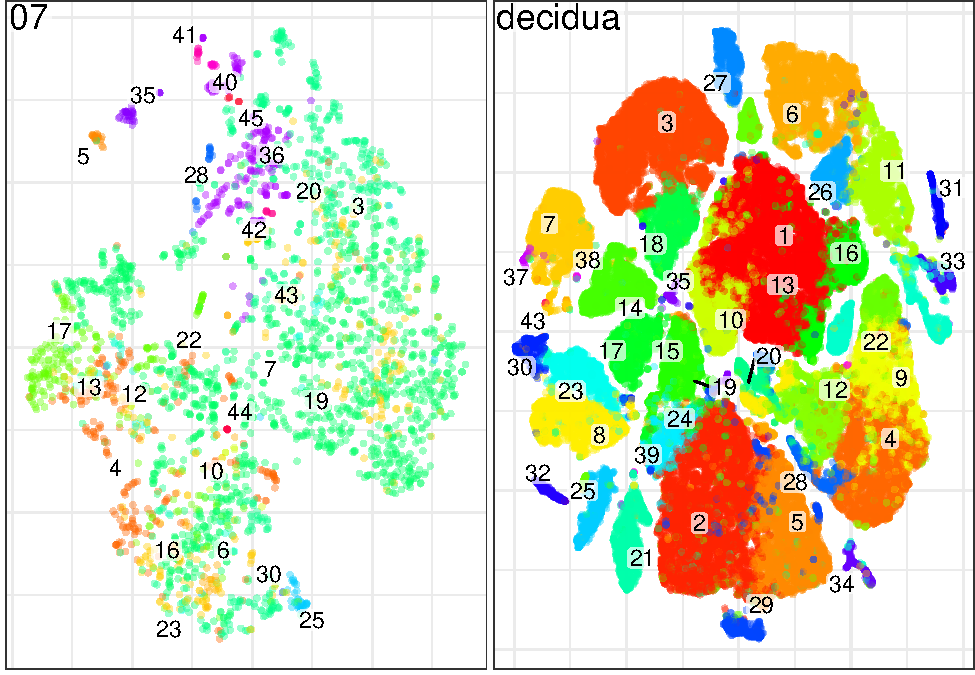
\includegraphics{labelling_integrated_files/figure-latex/unnamed-chunk-8-1.pdf}

\begin{Shaded}
\begin{Highlighting}[]
\NormalTok{con}\OperatorTok{$}\KeywordTok{buildGraph}\NormalTok{(}\DataTypeTok{k=}\DecValTok{30}\NormalTok{, }\DataTypeTok{k.self=}\DecValTok{5}\NormalTok{, }\DataTypeTok{space=}\StringTok{'PCA'}\NormalTok{, }\DataTypeTok{ncomps=}\DecValTok{30}\NormalTok{, }\DataTypeTok{n.odgenes=}\DecValTok{2000}\NormalTok{, }
               \DataTypeTok{matching.method=}\StringTok{'mNN'}\NormalTok{, }\DataTypeTok{metric=}\StringTok{'angular'}\NormalTok{, }
               \DataTypeTok{score.component.variance=}\OtherTok{TRUE}\NormalTok{, }\DataTypeTok{verbose=}\OtherTok{TRUE}\NormalTok{)}
\end{Highlighting}
\end{Shaded}

\begin{verbatim}
## found 0 out of 1 cached PCA  space pairs ... running 1 additional PCA  space pairs
\end{verbatim}

\begin{verbatim}
## Warning in scaledMatricesSeuratV3(so.objs = samples, data.type =
## data.type, : Seurat doesn't support variance scaling
\end{verbatim}

\begin{verbatim}
## . done
## inter-sample links using  mNN
\end{verbatim}

\begin{verbatim}
## Warning in scaledMatricesSeuratV3(so.objs = samples, data.type =
## data.type, : Seurat doesn't support variance scaling
\end{verbatim}

\begin{verbatim}
## . done
## local pairs local pairs  done
## building graph ..done
\end{verbatim}

\begin{Shaded}
\begin{Highlighting}[]
\NormalTok{con}\OperatorTok{$}\KeywordTok{findCommunities}\NormalTok{(}\DataTypeTok{method=}\NormalTok{leiden.community, }\DataTypeTok{resolution=}\DecValTok{1}\NormalTok{)}
\end{Highlighting}
\end{Shaded}

Clusters correspond between datasets

\begin{Shaded}
\begin{Highlighting}[]
\NormalTok{con}\OperatorTok{$}\KeywordTok{plotPanel}\NormalTok{(}\DataTypeTok{font.size=}\DecValTok{4}\NormalTok{)}
\end{Highlighting}
\end{Shaded}

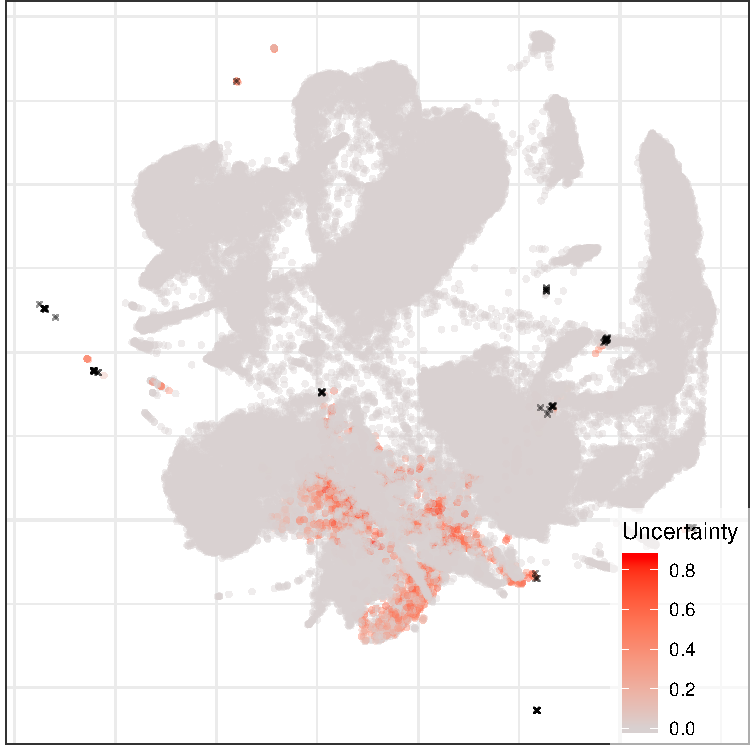
\includegraphics{labelling_integrated_files/figure-latex/unnamed-chunk-10-1.pdf}

\begin{Shaded}
\begin{Highlighting}[]
\NormalTok{cellannot <-}\StringTok{ }\NormalTok{seu_list[[}\StringTok{"decidua"}\NormalTok{]]}\OperatorTok{$}\NormalTok{annotation}

\CommentTok{# propagating labels from reference}
\NormalTok{new.label.probabilities <-}\StringTok{ }\NormalTok{con}\OperatorTok{$}\KeywordTok{propagateLabels}\NormalTok{(}\DataTypeTok{labels =}\NormalTok{ cellannot, }\DataTypeTok{verbose=}\NormalTok{T, }\DataTypeTok{fixed.initial.labels=}\NormalTok{T)}
\NormalTok{new.label.probabilities <-}\StringTok{ }\NormalTok{new.label.probabilities[}\KeywordTok{complete.cases}\NormalTok{(new.label.probabilities),]}
\end{Highlighting}
\end{Shaded}

\begin{Shaded}
\begin{Highlighting}[]
\CommentTok{#pdf(paste0("/icgc/dkfzlsdf/analysis/B210/Evelin/plots/",norm,"_uncertainty.pdf"))}
\NormalTok{con}\OperatorTok{$}\KeywordTok{plotGraph}\NormalTok{(}\DataTypeTok{colors=}\NormalTok{(}\DecValTok{1} \OperatorTok{-}\StringTok{ }\KeywordTok{apply}\NormalTok{(new.label.probabilities, }\DecValTok{1}\NormalTok{, max)), }\DataTypeTok{show.legend=}\NormalTok{T, }\DataTypeTok{legend.title=}\StringTok{"Uncertainty"}\NormalTok{, }\DataTypeTok{legend.pos=}\KeywordTok{c}\NormalTok{(}\DecValTok{1}\NormalTok{, }\DecValTok{0}\NormalTok{))}
\end{Highlighting}
\end{Shaded}

\begin{verbatim}
## Estimating embeddings.
\end{verbatim}

\includegraphics{labelling_integrated_files/figure-latex/unnamed-chunk-12-1.pdf}

\begin{Shaded}
\begin{Highlighting}[]
\CommentTok{#dev.off()}
\end{Highlighting}
\end{Shaded}

Clusters labelled based on reference

\begin{Shaded}
\begin{Highlighting}[]
\CommentTok{#pdf(paste0("/icgc/dkfzlsdf/analysis/B210/Evelin/plots/",norm,"_conos_labelled_clusters.pdf"))}
\NormalTok{con}\OperatorTok{$}\KeywordTok{plotPanel}\NormalTok{(}\DataTypeTok{groups =}\NormalTok{ new.annot)}
\end{Highlighting}
\end{Shaded}

\includegraphics{labelling_integrated_files/figure-latex/unnamed-chunk-14-1.pdf}

\begin{Shaded}
\begin{Highlighting}[]
\CommentTok{#dev.off()}
\end{Highlighting}
\end{Shaded}

Projecting conos predictions onto initial UMAP from Seurat

\begin{Shaded}
\begin{Highlighting}[]
\KeywordTok{DimPlot}\NormalTok{(seu_full, }\DataTypeTok{reduction =} \StringTok{"log.umap"}\NormalTok{, }\DataTypeTok{group.by =} \StringTok{"conos"}\NormalTok{, }\DataTypeTok{cells =} \KeywordTok{which}\NormalTok{(}\OperatorTok{!}\KeywordTok{is.na}\NormalTok{(seu_full}\OperatorTok{$}\NormalTok{conos)))}
\end{Highlighting}
\end{Shaded}

\includegraphics{labelling_integrated_files/figure-latex/unnamed-chunk-16-1.pdf}

\begin{Shaded}
\begin{Highlighting}[]
\KeywordTok{DimPlot}\NormalTok{(seu_full, }\DataTypeTok{reduction =} \StringTok{"log.umap"}\NormalTok{, }\DataTypeTok{group.by =} \StringTok{"conos"}\NormalTok{, }\DataTypeTok{cells =} \KeywordTok{which}\NormalTok{(seu_full}\OperatorTok{$}\NormalTok{conos }\OperatorTok\StringTok{ }\KeywordTok{c}\NormalTok{(}\StringTok{"SCT"}\NormalTok{, }\StringTok{"VCT"}\NormalTok{, }\StringTok{"EVT"}\NormalTok{, }\StringTok{"fFB1"}\NormalTok{, }\StringTok{"fFB2"}\NormalTok{))) }\OperatorTok{+}\StringTok{ }\KeywordTok{labs}\NormalTok{(}\DataTypeTok{title =} \StringTok{"predicted fetal cells"}\NormalTok{)}
\end{Highlighting}
\end{Shaded}

\includegraphics{labelling_integrated_files/figure-latex/unnamed-chunk-17-1.pdf}

\begin{Shaded}
\begin{Highlighting}[]
\KeywordTok{DimPlot}\NormalTok{(seu_full, }\DataTypeTok{reduction =} \StringTok{"log.umap"}\NormalTok{, }\DataTypeTok{group.by =} \StringTok{"conos"}\NormalTok{, }\DataTypeTok{cells =} \KeywordTok{which}\NormalTok{(}\OperatorTok{!}\NormalTok{(}\KeywordTok{is.na}\NormalTok{(seu_full}\OperatorTok{$}\NormalTok{conos) }\OperatorTok{|}\StringTok{ }\NormalTok{seu_full}\OperatorTok{$}\NormalTok{conos }\OperatorTok\StringTok{ }\KeywordTok{c}\NormalTok{(}\StringTok{"SCT"}\NormalTok{, }\StringTok{"VCT"}\NormalTok{, }\StringTok{"EVT"}\NormalTok{, }\StringTok{"fFB1"}\NormalTok{, }\StringTok{"fFB2"}\NormalTok{)))) }\OperatorTok{+}\StringTok{ }\KeywordTok{labs}\NormalTok{(}\DataTypeTok{title =} \StringTok{"predicted maternal cells"}\NormalTok{)}
\end{Highlighting}
\end{Shaded}

\includegraphics{labelling_integrated_files/figure-latex/unnamed-chunk-18-1.pdf}

\hypertarget{marker-gene-based-cluster-labels}{%
\section{Marker gene based cluster
labels}\label{marker-gene-based-cluster-labels}}

\begin{Shaded}
\begin{Highlighting}[]
\NormalTok{seu_full}\OperatorTok{$}\NormalTok{celltype =}\StringTok{ }\DecValTok{0}
\NormalTok{seu_full}\OperatorTok{$}\NormalTok{celltype[}\KeywordTok{which}\NormalTok{(seu_full}\OperatorTok{$}\NormalTok{SCT.clusters }\OperatorTok{==}\StringTok{ }\DecValTok{14} \OperatorTok{|}\StringTok{ }\NormalTok{seu_full}\OperatorTok{$}\NormalTok{log.clusters }\OperatorTok{==}\StringTok{ }\DecValTok{15}\NormalTok{) ]=}\StringTok{"endothelial"}
\NormalTok{seu_full}\OperatorTok{$}\NormalTok{celltype[}\KeywordTok{which}\NormalTok{(seu_full}\OperatorTok{$}\NormalTok{SCT.clusters }\OperatorTok\StringTok{ }\KeywordTok{c}\NormalTok{(}\DecValTok{0}\NormalTok{, }\DecValTok{2}\NormalTok{, }\DecValTok{3}\NormalTok{, }\DecValTok{6}\NormalTok{, }\DecValTok{9}\NormalTok{, }\DecValTok{12}\NormalTok{)) ]=}\StringTok{"epithelial"}
\NormalTok{seu_full}\OperatorTok{$}\NormalTok{celltype[}\KeywordTok{which}\NormalTok{(seu_full}\OperatorTok{$}\NormalTok{SCT.clusters }\OperatorTok\StringTok{ }\KeywordTok{c}\NormalTok{(}\DecValTok{1}\NormalTok{, }\DecValTok{5}\NormalTok{)) ]=}\StringTok{"stromal"}
\NormalTok{seu_full}\OperatorTok{$}\NormalTok{celltype[}\KeywordTok{which}\NormalTok{(seu_full}\OperatorTok{$}\NormalTok{SCT.clusters }\OperatorTok\StringTok{ }\KeywordTok{c}\NormalTok{(}\DecValTok{11}\NormalTok{)) ]=}\StringTok{"smooth muscle"}
\NormalTok{seu_full}\OperatorTok{$}\NormalTok{celltype[}\KeywordTok{which}\NormalTok{(seu_full}\OperatorTok{$}\NormalTok{celltype}\OperatorTok{==}\DecValTok{0}\NormalTok{) ]=}\OtherTok{NA}

\KeywordTok{plot_grid}\NormalTok{(}\KeywordTok{DimPlot}\NormalTok{(seu_full, }\DataTypeTok{reduction =} \StringTok{"log.umap"}\NormalTok{, }\DataTypeTok{group.by =} \StringTok{"celltype"}\NormalTok{, }\DataTypeTok{cells =} \KeywordTok{which}\NormalTok{(}\OperatorTok{!}\KeywordTok{is.na}\NormalTok{(seu_full}\OperatorTok{$}\NormalTok{celltype))), }\KeywordTok{DimPlot}\NormalTok{(seu_full, }\DataTypeTok{reduction =} \StringTok{"SCT.umap"}\NormalTok{, }\DataTypeTok{group.by =} \StringTok{"celltype"}\NormalTok{, }\DataTypeTok{cells =} \KeywordTok{which}\NormalTok{(}\OperatorTok{!}\KeywordTok{is.na}\NormalTok{(seu_full}\OperatorTok{$}\NormalTok{celltype))), }\KeywordTok{DimPlot}\NormalTok{(seu_full, }\DataTypeTok{reduction =} \StringTok{"integrated.umap"}\NormalTok{, }\DataTypeTok{group.by =} \StringTok{"celltype"}\NormalTok{, }\DataTypeTok{cells =} \KeywordTok{which}\NormalTok{(}\OperatorTok{!}\KeywordTok{is.na}\NormalTok{(seu_full}\OperatorTok{$}\NormalTok{celltype))), }\DataTypeTok{ncol =} \DecValTok{3}\NormalTok{)}
\end{Highlighting}
\end{Shaded}

\includegraphics{labelling_integrated_files/figure-latex/unnamed-chunk-19-1.pdf}

\begin{Shaded}
\begin{Highlighting}[]
\KeywordTok{DimPlot}\NormalTok{(seu_full, }\DataTypeTok{reduction =} \StringTok{"log.umap"}\NormalTok{, }\DataTypeTok{group.by =} \StringTok{"celltype"}\NormalTok{, }\DataTypeTok{cells =} \KeywordTok{which}\NormalTok{(}\OperatorTok{!}\KeywordTok{is.na}\NormalTok{(seu_full}\OperatorTok{$}\NormalTok{celltype)))}
\end{Highlighting}
\end{Shaded}

\includegraphics{labelling_integrated_files/figure-latex/unnamed-chunk-20-1.pdf}

\hypertarget{scmap}{%
\section{Scmap}\label{scmap}}

Scmap uses SingleCellExperiment objects as input

\begin{Shaded}
\begin{Highlighting}[]
\NormalTok{seu =}\StringTok{ }\NormalTok{seu_list[[}\StringTok{"menstrual"}\NormalTok{]]}
\NormalTok{rowData =}\StringTok{ }\KeywordTok{data.frame}\NormalTok{(}\DataTypeTok{feature_symbol =} \KeywordTok{row.names}\NormalTok{(seu[[assay]]))}
\NormalTok{colData =}\StringTok{ }\KeywordTok{data.frame}\NormalTok{(}\DataTypeTok{Barcode =} \KeywordTok{colnames}\NormalTok{(seu[[assay]]))}
\NormalTok{cluster_info =}\StringTok{ }\KeywordTok{data.frame}\NormalTok{(}\DataTypeTok{cluster =} \KeywordTok{Idents}\NormalTok{(seu))}
\NormalTok{cluster_info}\OperatorTok{$}\NormalTok{Barcode =}\StringTok{ }\KeywordTok{row.names}\NormalTok{(cluster_info)}
\NormalTok{colData =}\StringTok{ }\KeywordTok{left_join}\NormalTok{(colData, cluster_info, }\DataTypeTok{by =} \StringTok{"Barcode"}\NormalTok{)}
\end{Highlighting}
\end{Shaded}

\begin{verbatim}
## Warning: Column `Barcode` joining factor and character vector, coercing
## into character vector
\end{verbatim}

\begin{Shaded}
\begin{Highlighting}[]
\NormalTok{assays =}\StringTok{ }\KeywordTok{return_assay}\NormalTok{(seu, assay)}

\NormalTok{se =}\StringTok{ }\KeywordTok{SummarizedExperiment}\NormalTok{(}\DataTypeTok{assays =} \KeywordTok{list}\NormalTok{(}\DataTypeTok{counts =}\NormalTok{ assays[[}\DecValTok{1}\NormalTok{]], }\DataTypeTok{logcounts =}\NormalTok{ assays[[}\DecValTok{2}\NormalTok{]]), }\DataTypeTok{rowData =}\NormalTok{ rowData, }\DataTypeTok{colData =}\NormalTok{ colData)}

\KeywordTok{rm}\NormalTok{(seu)}
\NormalTok{menstrual =}\StringTok{ }\KeywordTok{as}\NormalTok{(se, }\StringTok{"SingleCellExperiment"}\NormalTok{)}
\end{Highlighting}
\end{Shaded}

\begin{Shaded}
\begin{Highlighting}[]
\KeywordTok{load}\NormalTok{(}\DataTypeTok{file =} \KeywordTok{paste0}\NormalTok{(}\StringTok{"/icgc/dkfzlsdf/analysis/B210/Evelin/sce_RData/"}\NormalTok{,norm,}\StringTok{"_decidua_5000.RData"}\NormalTok{))}
\end{Highlighting}
\end{Shaded}

Feature selection

\begin{Shaded}
\begin{Highlighting}[]
\NormalTok{decidua <-}\StringTok{ }\KeywordTok{selectFeatures}\NormalTok{(decidua, }\DataTypeTok{suppress_plot =} \OtherTok{FALSE}\NormalTok{, }\DecValTok{1000}\NormalTok{)}
\end{Highlighting}
\end{Shaded}

\includegraphics{labelling_integrated_files/figure-latex/unnamed-chunk-23-1.pdf}

\begin{Shaded}
\begin{Highlighting}[]
\NormalTok{decidua <-}\StringTok{ }\KeywordTok{indexCluster}\NormalTok{(decidua, }\DataTypeTok{cluster_col =} \StringTok{"annotation"}\NormalTok{)}
\end{Highlighting}
\end{Shaded}

Variable genes

\begin{Shaded}
\begin{Highlighting}[]
\CommentTok{#pdf(paste0("/icgc/dkfzlsdf/analysis/B210/Evelin/plots/",assay,"50_variable_decidua.pdf"))}
\KeywordTok{pheatmap}\NormalTok{(}\KeywordTok{metadata}\NormalTok{(decidua)}\OperatorTok{$}\NormalTok{scmap_cluster_index, }\DataTypeTok{show_rownames =} \OtherTok{FALSE}\NormalTok{)}
\end{Highlighting}
\end{Shaded}

\includegraphics{labelling_integrated_files/figure-latex/unnamed-chunk-24-1.pdf}

\begin{Shaded}
\begin{Highlighting}[]
\CommentTok{#dev.off()}
\end{Highlighting}
\end{Shaded}

Celltypes in reference dataset

\begin{Shaded}
\begin{Highlighting}[]
\NormalTok{df =}\StringTok{ }\KeywordTok{as.data.frame}\NormalTok{(}\KeywordTok{table}\NormalTok{(}\KeywordTok{colData}\NormalTok{(decidua)}\OperatorTok{$}\NormalTok{annotation))}
\KeywordTok{ggplot}\NormalTok{(df, }\KeywordTok{aes}\NormalTok{(}\DataTypeTok{x =} \KeywordTok{reorder}\NormalTok{(Var1, }\OperatorTok{-}\NormalTok{Freq), }\DataTypeTok{y =}\NormalTok{ Freq)) }\OperatorTok{+}\StringTok{ }\KeywordTok{geom_col}\NormalTok{() }\OperatorTok{+}\StringTok{ }
\StringTok{  }\KeywordTok{theme_bw}\NormalTok{() }\OperatorTok{+}\StringTok{ }\KeywordTok{theme}\NormalTok{(}\DataTypeTok{axis.text.x =} \KeywordTok{element_text}\NormalTok{(}\DataTypeTok{angle =} \DecValTok{45}\NormalTok{)) }\OperatorTok{+}\StringTok{ }
\StringTok{  }\KeywordTok{labs}\NormalTok{(}\DataTypeTok{title =} \StringTok{"decidua reference celltypes"}\NormalTok{)}
\end{Highlighting}
\end{Shaded}

\includegraphics{labelling_integrated_files/figure-latex/unnamed-chunk-26-1.pdf}

\begin{Shaded}
\begin{Highlighting}[]
\CommentTok{#ggsave(paste0("/icgc/dkfzlsdf/analysis/B210/Evelin/plots/",assay,"_reference_celltypes.pdf"))}
\end{Highlighting}
\end{Shaded}

\begin{Shaded}
\begin{Highlighting}[]
\NormalTok{df =}\StringTok{ }\KeywordTok{as.data.frame}\NormalTok{(}\KeywordTok{table}\NormalTok{(}\KeywordTok{as.data.frame}\NormalTok{(scmapCluster_results)}\OperatorTok{$}\NormalTok{decidua))}
\KeywordTok{ggplot}\NormalTok{(df, }\KeywordTok{aes}\NormalTok{(}\DataTypeTok{x =} \KeywordTok{reorder}\NormalTok{(Var1, }\OperatorTok{-}\NormalTok{Freq), }\DataTypeTok{y =}\NormalTok{ Freq)) }\OperatorTok{+}\StringTok{ }\KeywordTok{geom_col}\NormalTok{() }\OperatorTok{+}\StringTok{ }
\StringTok{  }\KeywordTok{theme_bw}\NormalTok{() }\OperatorTok{+}\StringTok{ }\KeywordTok{theme}\NormalTok{(}\DataTypeTok{axis.text.x =} \KeywordTok{element_text}\NormalTok{(}\DataTypeTok{angle =} \DecValTok{45}\NormalTok{)) }\OperatorTok{+}\StringTok{ }
\StringTok{  }\KeywordTok{labs}\NormalTok{(}\DataTypeTok{title =} \StringTok{"projected celltypes"}\NormalTok{)}
\end{Highlighting}
\end{Shaded}

\includegraphics{labelling_integrated_files/figure-latex/unnamed-chunk-27-1.pdf}

\begin{Shaded}
\begin{Highlighting}[]
\CommentTok{#ggsave(paste0("/icgc/dkfzlsdf/analysis/B210/Evelin/plots/",assay,"_celltypes_all_genes.pdf"))}
\end{Highlighting}
\end{Shaded}


\end{document}
